%============================================================
% RUNNER: BUKU PROYEK AKHIR
% Compile: pdflatex main_buku.tex (3x) + bibtex main_buku
% Output : main_buku.pdf
%
% Isi lengkap: cover, halaman judul, pengesahan, semua front
% matter, Bab 1-5, daftar pustaka, lampiran.
%============================================================

\documentclass[12pt, a4paper, twoside, openright, fleqn]{report}

% ── Konfigurasi (urutan penting) ─────────────────────────────
%============================================================
% VARIABEL IDENTITAS DOKUMEN
% Edit bagian ini sesuai dengan data proyek akhir Anda.
% File ini di-input pertama kali agar semua file lain
% dapat mereferensikan variabel-variabel berikut.
%============================================================

% ── Identitas Mahasiswa ──────────────────────────────────────
\newcommand{\NamaMahasiswa}{Nama Lengkap Mahasiswa}
\newcommand{\NRP}{xxxxxxxxxx}

% ── Judul Proyek Akhir ───────────────────────────────────────
% Tulis judul dengan kapitalisasi biasa; \MakeUppercase
% diterapkan secara otomatis di tempat yang membutuhkannya.
\newcommand{\JudulPA}{Lorem ipsum dolor sit amet, consectetur adipiscing elit.
Nam sed aliquam odio, eu congue ex. }

% ── Dosen Pembimbing (sertakan gelar akademis) ───────────────
\newcommand{\NamaPembimbingSatu}{Nama Lengkap dan Gelar}
\newcommand{\NIPPembimbingSatu}{xxxxxxxxxxxxxxxxxx}
\newcommand{\NamaPembimbingDua}{Nama Lengkap dan Gelar}
\newcommand{\NIPPembimbingDua}{xxxxxxxxxxxxxxxxxx}

% ── Dosen Penguji (sertakan gelar akademis) ──────────────────
\newcommand{\NamaPengujiSatu}{Nama Lengkap dan Gelar}
\newcommand{\NIPPengujiSatu}{xxxxxxxxxxxxxxx}
\newcommand{\NamaPengujiDua}{Nama Lengkap dan Gelar}
\newcommand{\NIPPengujiDua}{xxxxxxxxxxxxxxx}

% ── Pembimbing Opsional (Isi salah satu saja, atau kosongkan keduanya) ──
% Isi jika memiliki Dosen Pembimbing ke-3 (Akademik)
\newcommand{\NamaPembimbingTiga}{}
\newcommand{\NIPPembimbingTiga}{}

% Isi jika memiliki Pembimbing ke-3 dari luar (Dosen/Industri).
% Bisa berupa dosen tambahan (isi NIP) atau pembimbing industri (isi Perusahaan).
% Kosongkan keduanya jika tidak ada pembimbing tambahan.
\newcommand{\NamaPembimbingIndustri}{}  % Contoh: Nama Lengkap dan Gelar
\newcommand{\NIPPembimbingIndustri}{}   % Isi jika dosen (NIP), kosongkan jika industri
\newcommand{\NamaPerusahaanIndustri}{}  % Isi jika industri (contoh: PT. Nama Perusahaan), kosongkan jika dosen

% ── Ketua Program Studi (sertakan gelar akademis) ────────────
\newcommand{\NamaKetuaProdi}{Yanuar Risah Prayogi, S.Kom., M.Kom}
\newcommand{\NIPKetuaProdi}{198801062019031009}

% ── Program Studi & Institusi ────────────────────────────────
\newcommand{\NamaProdi}{Teknik Informatika}
\newcommand{\NamaDepartemen}{Departemen Teknik Informatika Dan Komputer}

% ── Gelar yang Diperoleh ─────────────────────────────────────
\newcommand{\GelarLulus}{Sarjana Terapan Komputer (S.Tr.Kom.)}

% ── Tahun Kelulusan ──────────────────────────────────────────
\newcommand{\TahunLulus}{2026}

% ── Tanggal Sidang ───────────────────────────────────────────
% Dipakai di halaman pernyataan. Format: Surabaya, DD Bulan YYYY
\newcommand{\TanggalSidang}{Surabaya, \today}

%============================================================
% TOGGLES: Boolean Switch Front Matter Opsional
% Default: FALSE, semua seksi opsional tidak ditampilkan.
% Override di main_*.tex jika diperlukan.
%============================================================

% Toggle Front Matter Opsional
% Set ke true untuk menampilkan seksi yang diinginkan.
\newif\ifshowabstrak       \showabstrakfalse       % Abstrak (ID)
\newif\ifshowabstract      \showabstractfalse      % Abstract (EN)
\newif\ifshowkatapengantar \showkatapengantarfalse % Kata Pengantar
\newif\ifshowdaftarisi     \showdaftarisifalse     % Daftar Isi
\newif\ifshowdaftargambar  \showdaftargambarfalse  % Daftar Gambar
\newif\ifshowdaftartabel   \showdaftartabelfalse   % Daftar Tabel

% Toggle Paksa Halaman Ganjil
% Jika true, setiap bab dan seksi front matter selalu dimulai
% di halaman ganjil (sisipkan halaman kosong jika perlu).
% Buku PA: aktif otomatis (openright).
% Proposal & Progres: default false (oneside, tidak memerlukan ini).
% Aktifkan dengan menambahkan \showforceoddpagetrue di main_*.tex.
\newif\ifshowforceoddpage  \showforceoddpagefalse

% Toggle Jenis Dokumen: Buku PA
% true  -> Buku PA (ada Batasan Masalah di Bab 1, seksi lengkap)
% false -> Proposal / Progres (tanpa Batasan Masalah)
% Diset true di main_buku.tex sebelum %============================================================
% TOGGLES: Boolean Switch Front Matter Opsional
% Default: FALSE, semua seksi opsional tidak ditampilkan.
% Override di main_*.tex jika diperlukan.
%============================================================

% Toggle Front Matter Opsional
% Set ke true untuk menampilkan seksi yang diinginkan.
\newif\ifshowabstrak       \showabstrakfalse       % Abstrak (ID)
\newif\ifshowabstract      \showabstractfalse      % Abstract (EN)
\newif\ifshowkatapengantar \showkatapengantarfalse % Kata Pengantar
\newif\ifshowdaftarisi     \showdaftarisifalse     % Daftar Isi
\newif\ifshowdaftargambar  \showdaftargambarfalse  % Daftar Gambar
\newif\ifshowdaftartabel   \showdaftartabelfalse   % Daftar Tabel

% Toggle Paksa Halaman Ganjil
% Jika true, setiap bab dan seksi front matter selalu dimulai
% di halaman ganjil (sisipkan halaman kosong jika perlu).
% Buku PA: aktif otomatis (openright).
% Proposal & Progres: default false (oneside, tidak memerlukan ini).
% Aktifkan dengan menambahkan \showforceoddpagetrue di main_*.tex.
\newif\ifshowforceoddpage  \showforceoddpagefalse

% Toggle Jenis Dokumen: Buku PA
% true  -> Buku PA (ada Batasan Masalah di Bab 1, seksi lengkap)
% false -> Proposal / Progres (tanpa Batasan Masalah)
% Diset true di main_buku.tex sebelum %============================================================
% TOGGLES: Boolean Switch Front Matter Opsional
% Default: FALSE, semua seksi opsional tidak ditampilkan.
% Override di main_*.tex jika diperlukan.
%============================================================

% Toggle Front Matter Opsional
% Set ke true untuk menampilkan seksi yang diinginkan.
\newif\ifshowabstrak       \showabstrakfalse       % Abstrak (ID)
\newif\ifshowabstract      \showabstractfalse      % Abstract (EN)
\newif\ifshowkatapengantar \showkatapengantarfalse % Kata Pengantar
\newif\ifshowdaftarisi     \showdaftarisifalse     % Daftar Isi
\newif\ifshowdaftargambar  \showdaftargambarfalse  % Daftar Gambar
\newif\ifshowdaftartabel   \showdaftartabelfalse   % Daftar Tabel

% Toggle Paksa Halaman Ganjil
% Jika true, setiap bab dan seksi front matter selalu dimulai
% di halaman ganjil (sisipkan halaman kosong jika perlu).
% Buku PA: aktif otomatis (openright).
% Proposal & Progres: default false (oneside, tidak memerlukan ini).
% Aktifkan dengan menambahkan \showforceoddpagetrue di main_*.tex.
\newif\ifshowforceoddpage  \showforceoddpagefalse

% Toggle Jenis Dokumen: Buku PA
% true  -> Buku PA (ada Batasan Masalah di Bab 1, seksi lengkap)
% false -> Proposal / Progres (tanpa Batasan Masalah)
% Diset true di main_buku.tex sebelum \input{config/toggles}.
\newif\ifbukupa            \bukupafalse

% ── Toggle Khusus Buku PA ─────────────────────────────────────
% Aktifkan di main_buku.tex (setelah \input{config/toggles}).

% Sisipkan lembar pengesahan PDF yang sudah ditandatangani,
% menggantikan halaman pengesahan hasil generate LaTeX.
\newif\ifpengesahanpdf     \pengesahanpdffalse
\newcommand{\FilePengesahanPDF}{pages/lembar_pengesahan.pdf}

% Sisipkan PDF pernyataan pengalihan hak cipta yang sudah
% ditandatangani di atas materai.
\newif\ifhakciptapdf       \hakciptapdffalse
\newcommand{\FileHakCiptaPDF}{pages/hak_cipta_materai.pdf}

% Mode Digilib (upload repository / berkas yudisium):
% true  -> watermark PENS aktif mulai Abstrak, TANPA halaman
%          "sengaja dikosongkan" (file nanti dipotong per bagian)
% false -> versi cetak biasa (default)
% Bisa juga lewat `make digilib` tanpa mengedit file.
\newif\ifdigilib           \digilibfalse

% Halaman Biodata Penulis di akhir Buku PA (default: tidak ditampilkan).
% Aktifkan dengan \showbiodatatrue di main_buku.tex.
\newif\ifshowbiodata       \showbiodatafalse
.
\newif\ifbukupa            \bukupafalse

% ── Toggle Khusus Buku PA ─────────────────────────────────────
% Aktifkan di main_buku.tex (setelah %============================================================
% TOGGLES: Boolean Switch Front Matter Opsional
% Default: FALSE, semua seksi opsional tidak ditampilkan.
% Override di main_*.tex jika diperlukan.
%============================================================

% Toggle Front Matter Opsional
% Set ke true untuk menampilkan seksi yang diinginkan.
\newif\ifshowabstrak       \showabstrakfalse       % Abstrak (ID)
\newif\ifshowabstract      \showabstractfalse      % Abstract (EN)
\newif\ifshowkatapengantar \showkatapengantarfalse % Kata Pengantar
\newif\ifshowdaftarisi     \showdaftarisifalse     % Daftar Isi
\newif\ifshowdaftargambar  \showdaftargambarfalse  % Daftar Gambar
\newif\ifshowdaftartabel   \showdaftartabelfalse   % Daftar Tabel

% Toggle Paksa Halaman Ganjil
% Jika true, setiap bab dan seksi front matter selalu dimulai
% di halaman ganjil (sisipkan halaman kosong jika perlu).
% Buku PA: aktif otomatis (openright).
% Proposal & Progres: default false (oneside, tidak memerlukan ini).
% Aktifkan dengan menambahkan \showforceoddpagetrue di main_*.tex.
\newif\ifshowforceoddpage  \showforceoddpagefalse

% Toggle Jenis Dokumen: Buku PA
% true  -> Buku PA (ada Batasan Masalah di Bab 1, seksi lengkap)
% false -> Proposal / Progres (tanpa Batasan Masalah)
% Diset true di main_buku.tex sebelum \input{config/toggles}.
\newif\ifbukupa            \bukupafalse

% ── Toggle Khusus Buku PA ─────────────────────────────────────
% Aktifkan di main_buku.tex (setelah \input{config/toggles}).

% Sisipkan lembar pengesahan PDF yang sudah ditandatangani,
% menggantikan halaman pengesahan hasil generate LaTeX.
\newif\ifpengesahanpdf     \pengesahanpdffalse
\newcommand{\FilePengesahanPDF}{pages/lembar_pengesahan.pdf}

% Sisipkan PDF pernyataan pengalihan hak cipta yang sudah
% ditandatangani di atas materai.
\newif\ifhakciptapdf       \hakciptapdffalse
\newcommand{\FileHakCiptaPDF}{pages/hak_cipta_materai.pdf}

% Mode Digilib (upload repository / berkas yudisium):
% true  -> watermark PENS aktif mulai Abstrak, TANPA halaman
%          "sengaja dikosongkan" (file nanti dipotong per bagian)
% false -> versi cetak biasa (default)
% Bisa juga lewat `make digilib` tanpa mengedit file.
\newif\ifdigilib           \digilibfalse

% Halaman Biodata Penulis di akhir Buku PA (default: tidak ditampilkan).
% Aktifkan dengan \showbiodatatrue di main_buku.tex.
\newif\ifshowbiodata       \showbiodatafalse
).

% Sisipkan lembar pengesahan PDF yang sudah ditandatangani,
% menggantikan halaman pengesahan hasil generate LaTeX.
\newif\ifpengesahanpdf     \pengesahanpdffalse
\newcommand{\FilePengesahanPDF}{pages/lembar_pengesahan.pdf}

% Sisipkan PDF pernyataan pengalihan hak cipta yang sudah
% ditandatangani di atas materai.
\newif\ifhakciptapdf       \hakciptapdffalse
\newcommand{\FileHakCiptaPDF}{pages/hak_cipta_materai.pdf}

% Mode Digilib (upload repository / berkas yudisium):
% true  -> watermark PENS aktif mulai Abstrak, TANPA halaman
%          "sengaja dikosongkan" (file nanti dipotong per bagian)
% false -> versi cetak biasa (default)
% Bisa juga lewat `make digilib` tanpa mengedit file.
\newif\ifdigilib           \digilibfalse

% Halaman Biodata Penulis di akhir Buku PA (default: tidak ditampilkan).
% Aktifkan dengan \showbiodatatrue di main_buku.tex.
\newif\ifshowbiodata       \showbiodatafalse
.
\newif\ifbukupa            \bukupafalse

% ── Toggle Khusus Buku PA ─────────────────────────────────────
% Aktifkan di main_buku.tex (setelah %============================================================
% TOGGLES: Boolean Switch Front Matter Opsional
% Default: FALSE, semua seksi opsional tidak ditampilkan.
% Override di main_*.tex jika diperlukan.
%============================================================

% Toggle Front Matter Opsional
% Set ke true untuk menampilkan seksi yang diinginkan.
\newif\ifshowabstrak       \showabstrakfalse       % Abstrak (ID)
\newif\ifshowabstract      \showabstractfalse      % Abstract (EN)
\newif\ifshowkatapengantar \showkatapengantarfalse % Kata Pengantar
\newif\ifshowdaftarisi     \showdaftarisifalse     % Daftar Isi
\newif\ifshowdaftargambar  \showdaftargambarfalse  % Daftar Gambar
\newif\ifshowdaftartabel   \showdaftartabelfalse   % Daftar Tabel

% Toggle Paksa Halaman Ganjil
% Jika true, setiap bab dan seksi front matter selalu dimulai
% di halaman ganjil (sisipkan halaman kosong jika perlu).
% Buku PA: aktif otomatis (openright).
% Proposal & Progres: default false (oneside, tidak memerlukan ini).
% Aktifkan dengan menambahkan \showforceoddpagetrue di main_*.tex.
\newif\ifshowforceoddpage  \showforceoddpagefalse

% Toggle Jenis Dokumen: Buku PA
% true  -> Buku PA (ada Batasan Masalah di Bab 1, seksi lengkap)
% false -> Proposal / Progres (tanpa Batasan Masalah)
% Diset true di main_buku.tex sebelum %============================================================
% TOGGLES: Boolean Switch Front Matter Opsional
% Default: FALSE, semua seksi opsional tidak ditampilkan.
% Override di main_*.tex jika diperlukan.
%============================================================

% Toggle Front Matter Opsional
% Set ke true untuk menampilkan seksi yang diinginkan.
\newif\ifshowabstrak       \showabstrakfalse       % Abstrak (ID)
\newif\ifshowabstract      \showabstractfalse      % Abstract (EN)
\newif\ifshowkatapengantar \showkatapengantarfalse % Kata Pengantar
\newif\ifshowdaftarisi     \showdaftarisifalse     % Daftar Isi
\newif\ifshowdaftargambar  \showdaftargambarfalse  % Daftar Gambar
\newif\ifshowdaftartabel   \showdaftartabelfalse   % Daftar Tabel

% Toggle Paksa Halaman Ganjil
% Jika true, setiap bab dan seksi front matter selalu dimulai
% di halaman ganjil (sisipkan halaman kosong jika perlu).
% Buku PA: aktif otomatis (openright).
% Proposal & Progres: default false (oneside, tidak memerlukan ini).
% Aktifkan dengan menambahkan \showforceoddpagetrue di main_*.tex.
\newif\ifshowforceoddpage  \showforceoddpagefalse

% Toggle Jenis Dokumen: Buku PA
% true  -> Buku PA (ada Batasan Masalah di Bab 1, seksi lengkap)
% false -> Proposal / Progres (tanpa Batasan Masalah)
% Diset true di main_buku.tex sebelum \input{config/toggles}.
\newif\ifbukupa            \bukupafalse

% ── Toggle Khusus Buku PA ─────────────────────────────────────
% Aktifkan di main_buku.tex (setelah \input{config/toggles}).

% Sisipkan lembar pengesahan PDF yang sudah ditandatangani,
% menggantikan halaman pengesahan hasil generate LaTeX.
\newif\ifpengesahanpdf     \pengesahanpdffalse
\newcommand{\FilePengesahanPDF}{pages/lembar_pengesahan.pdf}

% Sisipkan PDF pernyataan pengalihan hak cipta yang sudah
% ditandatangani di atas materai.
\newif\ifhakciptapdf       \hakciptapdffalse
\newcommand{\FileHakCiptaPDF}{pages/hak_cipta_materai.pdf}

% Mode Digilib (upload repository / berkas yudisium):
% true  -> watermark PENS aktif mulai Abstrak, TANPA halaman
%          "sengaja dikosongkan" (file nanti dipotong per bagian)
% false -> versi cetak biasa (default)
% Bisa juga lewat `make digilib` tanpa mengedit file.
\newif\ifdigilib           \digilibfalse

% Halaman Biodata Penulis di akhir Buku PA (default: tidak ditampilkan).
% Aktifkan dengan \showbiodatatrue di main_buku.tex.
\newif\ifshowbiodata       \showbiodatafalse
.
\newif\ifbukupa            \bukupafalse

% ── Toggle Khusus Buku PA ─────────────────────────────────────
% Aktifkan di main_buku.tex (setelah %============================================================
% TOGGLES: Boolean Switch Front Matter Opsional
% Default: FALSE, semua seksi opsional tidak ditampilkan.
% Override di main_*.tex jika diperlukan.
%============================================================

% Toggle Front Matter Opsional
% Set ke true untuk menampilkan seksi yang diinginkan.
\newif\ifshowabstrak       \showabstrakfalse       % Abstrak (ID)
\newif\ifshowabstract      \showabstractfalse      % Abstract (EN)
\newif\ifshowkatapengantar \showkatapengantarfalse % Kata Pengantar
\newif\ifshowdaftarisi     \showdaftarisifalse     % Daftar Isi
\newif\ifshowdaftargambar  \showdaftargambarfalse  % Daftar Gambar
\newif\ifshowdaftartabel   \showdaftartabelfalse   % Daftar Tabel

% Toggle Paksa Halaman Ganjil
% Jika true, setiap bab dan seksi front matter selalu dimulai
% di halaman ganjil (sisipkan halaman kosong jika perlu).
% Buku PA: aktif otomatis (openright).
% Proposal & Progres: default false (oneside, tidak memerlukan ini).
% Aktifkan dengan menambahkan \showforceoddpagetrue di main_*.tex.
\newif\ifshowforceoddpage  \showforceoddpagefalse

% Toggle Jenis Dokumen: Buku PA
% true  -> Buku PA (ada Batasan Masalah di Bab 1, seksi lengkap)
% false -> Proposal / Progres (tanpa Batasan Masalah)
% Diset true di main_buku.tex sebelum \input{config/toggles}.
\newif\ifbukupa            \bukupafalse

% ── Toggle Khusus Buku PA ─────────────────────────────────────
% Aktifkan di main_buku.tex (setelah \input{config/toggles}).

% Sisipkan lembar pengesahan PDF yang sudah ditandatangani,
% menggantikan halaman pengesahan hasil generate LaTeX.
\newif\ifpengesahanpdf     \pengesahanpdffalse
\newcommand{\FilePengesahanPDF}{pages/lembar_pengesahan.pdf}

% Sisipkan PDF pernyataan pengalihan hak cipta yang sudah
% ditandatangani di atas materai.
\newif\ifhakciptapdf       \hakciptapdffalse
\newcommand{\FileHakCiptaPDF}{pages/hak_cipta_materai.pdf}

% Mode Digilib (upload repository / berkas yudisium):
% true  -> watermark PENS aktif mulai Abstrak, TANPA halaman
%          "sengaja dikosongkan" (file nanti dipotong per bagian)
% false -> versi cetak biasa (default)
% Bisa juga lewat `make digilib` tanpa mengedit file.
\newif\ifdigilib           \digilibfalse

% Halaman Biodata Penulis di akhir Buku PA (default: tidak ditampilkan).
% Aktifkan dengan \showbiodatatrue di main_buku.tex.
\newif\ifshowbiodata       \showbiodatafalse
).

% Sisipkan lembar pengesahan PDF yang sudah ditandatangani,
% menggantikan halaman pengesahan hasil generate LaTeX.
\newif\ifpengesahanpdf     \pengesahanpdffalse
\newcommand{\FilePengesahanPDF}{pages/lembar_pengesahan.pdf}

% Sisipkan PDF pernyataan pengalihan hak cipta yang sudah
% ditandatangani di atas materai.
\newif\ifhakciptapdf       \hakciptapdffalse
\newcommand{\FileHakCiptaPDF}{pages/hak_cipta_materai.pdf}

% Mode Digilib (upload repository / berkas yudisium):
% true  -> watermark PENS aktif mulai Abstrak, TANPA halaman
%          "sengaja dikosongkan" (file nanti dipotong per bagian)
% false -> versi cetak biasa (default)
% Bisa juga lewat `make digilib` tanpa mengedit file.
\newif\ifdigilib           \digilibfalse

% Halaman Biodata Penulis di akhir Buku PA (default: tidak ditampilkan).
% Aktifkan dengan \showbiodatatrue di main_buku.tex.
\newif\ifshowbiodata       \showbiodatafalse
).

% Sisipkan lembar pengesahan PDF yang sudah ditandatangani,
% menggantikan halaman pengesahan hasil generate LaTeX.
\newif\ifpengesahanpdf     \pengesahanpdffalse
\newcommand{\FilePengesahanPDF}{pages/lembar_pengesahan.pdf}

% Sisipkan PDF pernyataan pengalihan hak cipta yang sudah
% ditandatangani di atas materai.
\newif\ifhakciptapdf       \hakciptapdffalse
\newcommand{\FileHakCiptaPDF}{pages/hak_cipta_materai.pdf}

% Mode Digilib (upload repository / berkas yudisium):
% true  -> watermark PENS aktif mulai Abstrak, TANPA halaman
%          "sengaja dikosongkan" (file nanti dipotong per bagian)
% false -> versi cetak biasa (default)
% Bisa juga lewat `make digilib` tanpa mengedit file.
\newif\ifdigilib           \digilibfalse

% Halaman Biodata Penulis di akhir Buku PA (default: tidak ditampilkan).
% Aktifkan dengan \showbiodatatrue di main_buku.tex.
\newif\ifshowbiodata       \showbiodatafalse


% ── Aktifkan khusus Buku PA ───────────────────────────────────
\bukupatrue   % Tampilkan Batasan Masalah di Bab 1

% ── Opsi Buku PA (uncomment untuk mengaktifkan) ───────────────
% \pengesahanpdftrue  % Pakai PDF pengesahan bertanda tangan (pages/lembar_pengesahan.pdf)
% \hakciptapdftrue    % Pakai PDF hak cipta bermaterai (pages/hak_cipta_materai.pdf)
% \digilibtrue        % Mode Digilib: watermark + tanpa halaman kosong (atau: make digilib)
% \showbiodatatrue    % Tampilkan halaman Biodata Penulis di akhir buku (pages/biodata.tex)

% `make digilib` meng-compile main_buku_digilib.tex yang mendefinisikan \ModeDigilib
\ifdefined\ModeDigilib \digilibtrue\fi

%============================================================
% PACKAGES
% Semua package yang digunakan dalam dokumen ini.
%============================================================

\usepackage[T1]{fontenc}
\usepackage[utf8]{inputenc}
\usepackage{mathptmx}    % Font Times New Roman (teks + math)
\usepackage{setspace}    % Pengaturan spasi baris
\usepackage{geometry}    % Pengaturan margin halaman
\usepackage{graphicx}    % Penyisipan gambar
\usepackage{caption}     % Kustomisasi caption gambar/tabel
\usepackage{float}       % Kontrol posisi float [H]
\usepackage{tabularx}    % Tabel dengan lebar kolom fleksibel
\usepackage{booktabs}    % Tabel bergaya profesional
\usepackage{array}       % Definisi kolom tabel kustom
\usepackage{amsmath}     % Persamaan matematika
\usepackage{amssymb}     % Simbol matematika tambahan
\usepackage{xcolor}      % Definisi warna
\usepackage{colortbl}    % Warna sel tabel (\rowcolor)
\usepackage{tikz}        % Grafis vektor (watermark, dll.)
\usepackage{fancyhdr}    % Header dan footer kustom
\usepackage{emptypage}   % Halaman kosong tanpa header/footer
\usepackage{tocloft}     % Kustomisasi Daftar Isi/Gambar/Tabel
\usepackage{titlesec}    % Format judul bab dan subbab
\usepackage{indentfirst} % Indentasi pada paragraf pertama
\usepackage{parskip}     % Pengaturan jarak antar paragraf
\usepackage{cite}        % Sitasi gaya IEEE
\usepackage{url}         % URL pada daftar pustaka
\usepackage{hyperref}    % Hyperlink internal/eksternal
\usepackage{ragged2e}    % Perataan teks fleksibel
\usepackage{microtype}   % Perbaikan tipografi mikro
\usepackage{enumitem}    % Kustomisasi list/enumerate
\usepackage{pdfpages}    % Menyisipkan halaman PDF eksternal
\usepackage{etoolbox}    % Utilitas pemrograman LaTeX
\usepackage{tabularray}  % Tabel modern (tblr, longtblr)
\usepackage{eso-pic}     % Untuk kontrol watermark background per halaman
\usepackage[indonesian]{babel} % Aturan hyphenation/pemenggalan kata Bahasa Indonesia
%============================================================
% UKURAN FONT
% Semua ukuran font template ada di sini. Ubah satu baris,
% berlaku di semua halaman yang memakai peran tersebut.
%
% Format: \fontsize{ukuran huruf}{jarak baris}\selectfont (pt)
% Nilai di bawah adalah ukuran Buku PA. Proposal & Progres
% meng-override sebagian lewat \renewcommand di
% formats/format_proposal.tex dan formats/format_progres.tex.
%
% Di-input setelah config/packages.tex dan sebelum
% config/formatting.tex di setiap main_*.tex.
%============================================================

% ── Judul Isi Dokumen (Buku PA; Proposal/Progres: 12pt) ──────
\newcommand{\FontJudulBab}{\fontsize{14}{17}\selectfont}           % BAB n + judul bab
\newcommand{\FontJudulSubbab}{\fontsize{14}{17}\selectfont}        % 1.1 (section)
\newcommand{\FontJudulSubSubbab}{\fontsize{12}{14}\selectfont}     % 1.1.1 (subsection)
\newcommand{\FontJudulSubSubSubbab}{\fontsize{12}{14}\selectfont}  % tanpa nomor (subsubsection)
\newcommand{\FontJudulDaftar}{\fontsize{14}{17}\selectfont}        % DAFTAR ISI / GAMBAR / TABEL
\newcommand{\FontKutipanPanjang}{\fontsize{10}{12}\selectfont}     % lingkungan kutipanpanjang
\newcommand{\FontSumber}{\fontsize{12}{15}\selectfont}             % "Sumber: ..." di bawah gambar/tabel

% ── Cover Buku PA (formats/cover_buku.tex) ───────────────────
\newcommand{\FontCoverBukuLabel}{\fontsize{20}{24}\selectfont}     % "PROYEK AKHIR"
\newcommand{\FontCoverBukuJudul}{\fontsize{18}{20}\selectfont}     % judul PA
\newcommand{\FontCoverBukuIsi}{\fontsize{16}{20}\selectfont}       % nama, NRP, pembimbing, prodi

% ── Halaman Judul Dalam Buku PA (formats/halaman_judul.tex) ──
\newcommand{\FontJudulDalamLabel}{\fontsize{20}{0}\selectfont}     % "PROYEK AKHIR"
\newcommand{\FontJudulDalamJudul}{\fontsize{18}{20}\selectfont}    % judul PA
\newcommand{\FontJudulDalamIsi}{\fontsize{16}{20}\selectfont}      % nama, NRP, pembimbing, prodi

% ── Halaman Pengesahan (formats/pengesahan.tex) ──────────────
\newcommand{\FontPengesahanLabel}{\fontsize{20}{0}\selectfont}     % "HALAMAN PENGESAHAN"
\newcommand{\FontPengesahanJudul}{\fontsize{18}{16}\selectfont}    % judul PA
\newcommand{\FontPengesahanIsi}{\fontsize{14}{17}\selectfont}      % isi & tabel tanda tangan

% ── Halaman Pernyataan (orisinalitas, hak cipta) ─────────────
\newcommand{\FontPernyataanLabel}{\fontsize{20}{10}\selectfont}    % judul halaman pernyataan
\newcommand{\FontPernyataanIsi}{\fontsize{12}{15}\selectfont}      % isi pernyataan orisinalitas

% ── Cover Proposal & Progres (formats/cover_proposal|progres.tex) ──
\newcommand{\FontCoverRingkasLabel}{\fontsize{20}{24}\selectfont}       % "PROPOSAL/PROGRES PROYEK AKHIR"
\newcommand{\FontCoverRingkasIsi}{\fontsize{18}{22}\selectfont}         % judul, nama, NRP, prodi
\newcommand{\FontCoverRingkasPembimbing}{\fontsize{18}{20}\selectfont}  % nama & NIP pembimbing

% Catatan: label 20pt memakai jarak baris berbeda (24pt di cover,
% 0pt di halaman judul & pengesahan, 10pt di halaman pernyataan).
% Nilai ini dipertahankan apa adanya agar hasil PDF tidak berubah.
% Jarak baris hanya berpengaruh jika judul tersebut lebih dari 1 baris.
         % ukuran font per peran
%============================================================
% FORMATTING: BASE LAYER (SHARED)
% Aturan yang 100% sama di Proposal, Progres, dan Buku PA.
% Aturan per-dokumen (geometry, spacing) ada di formats/format_*.tex
% yang di-input SETELAH file ini di masing-masing main_*.tex.
%============================================================

% ── Warna Institusi ──────────────────────────────────────────
\definecolor{pensbiru}{RGB}{0, 47, 167}    % Biru PENS (#002FA7)
\definecolor{penskuning}{RGB}{255, 193, 7} % Kuning/emas garis cover

% ── Indentasi & Paragraf ─────────────────────────────────────
% \parindent TIDAK diset di sini — tiap dokumen punya nilai sendiri:
%   Buku PA  : 1.27cm (ada di formats/format_buku.tex)
%   Proposal : 0.75cm (ada di formats/format_proposal.tex)
%   Progres  : 0.75cm (ada di formats/format_progres.tex)
\setlength{\parskip}{0pt}

% ── Persamaan Matematika ─────────────────────────────────────
\setlength{\mathindent}{10mm}
\setlength{\abovedisplayskip}{12pt}
\setlength{\belowdisplayskip}{12pt}
\setlength{\abovedisplayshortskip}{12pt}
\setlength{\belowdisplayshortskip}{12pt}

% Nomor persamaan dicetak tebal-miring
\makeatletter
\renewcommand{\tagform@}[1]{\maketag@@@{\bfseries\itshape(#1)\@@italiccorr}}
\makeatother

% ── Format Judul Bab ─────────────────────────────────────────
\titleformat{\chapter}[display]
{\centering\FontJudulBab\bfseries}
{BAB \thechapter}
{0pt}
{}
\titlespacing*{\chapter}{0pt}{-20pt}{18pt}

% ── Auto-selaraskan indentasi paragraf pertama dengan huruf judul (bukan nomor) ──
\newsavebox{\KotakLabelJudul}
\newdimen\LebarLabelJudul
\newcommand{\SelaraskanIndentAsli}[1]{%
  \sbox{\KotakLabelJudul}{#1}%
  \global\LebarLabelJudul=\wd\KotakLabelJudul
  \global\advance\LebarLabelJudul by 1em
  \xdef\ParindentAsliTersimpan{\the\parindent}%
  \global\parindent=\LebarLabelJudul
  \global\everypar{\parindent=\ParindentAsliTersimpan\relax\global\everypar{}}%
}

% ── Format Judul Subbab (Section) ────────────────────────────
\titleformat{\section}
{\FontJudulSubbab\bfseries}
{\thesection}
{1em}
{}
[\SelaraskanIndentAsli{\thesection}]
\titlespacing*{\section}{0pt}{15pt}{0pt}

% ── Format Judul Sub-subbab (Subsection) ─────────────────────
\titleformat{\subsection}
{\FontJudulSubSubbab\bfseries}
{\thesubsection}
{1em}
{}
[\SelaraskanIndentAsli{\thesubsection}]
\titlespacing*{\subsection}{0pt}{8pt}{3pt}

% ── Batas Penomoran dan Daftar Isi ───────────────────────────
% 0 = Chapter, 1 = Section, 2 = Subsection, 3 = Subsubsection
\setcounter{secnumdepth}{2}
\setcounter{tocdepth}{2}

% ── Format Judul Sub-sub-subbab (Subsubsection) ──────────────
% Tanpa nomor (secnumdepth=2) — heading ringan, spacing kecil.
% Label dikosongkan, sep 0pt, left=\parindent agar indent konsisten.
\titleformat{\subsubsection}
{\FontJudulSubSubSubbab\bfseries}
{}
{0pt}
{}
\titlespacing*{\subsubsection}{\parindent}{3pt}{2pt}

% ── Caption Gambar ───────────────────────────────────────────
\captionsetup[figure]{
  labelfont     = {it},
  textfont      = {it},
  font          = {small},   % ~11pt dalam dokumen 12pt
  justification = centering,
  skip          = 6pt,
  name          = Gambar,
  labelsep      = space
}

% ── Caption Tabel ────────────────────────────────────────────
\captionsetup[table]{
  labelfont     = {it},
  textfont      = {it},
  font          = {small},
  justification = centering,
  skip          = 6pt,
  position      = above,
  name          = Tabel,
  labelsep      = space
}
\renewcommand{\tablename}{Tabel}

% ── Format Default Tabularray ────────────────────────────────
% Berlaku untuk semua lingkungan tblr dan longtblr
\SetTblrInner{
  hlines, vlines,                                             % Garis kotak otomatis
  row{1} = {bg=gray!20, font=\bfseries, halign=c},           % Header: abu-abu, bold, center
  rowhead = 1,                                               % Ulangi header jika tabel terpotong halaman
}

\SetTblrInner[longtblr]{
  hlines, vlines,
  row{1} = {bg=gray!20, font=\bfseries, halign=c},
  rowhead = 1,
}

% ── Isi Tabel: 11pt, Spasi 1 ─────────────────────────────────
% Isi sel tblr/longtblr memakai \small (±11pt pada dokumen 12pt) dan
% spasi 1, tidak ikut spasi teks isi (1.5 / 1.15). Berlaku untuk
% Buku PA, Proposal, dan Progres. Caption tabel tidak terpengaruh.
\AddToHook{env/tblr/begin}{\small\linespread{1}\selectfont}
\AddToHook{env/longtblr/begin}{\small\linespread{1}\selectfont}

% ── Kustomisasi Khusus longtblr ──────────────────────────────
% 1. Menyamakan format caption longtblr dengan tabel biasa (Italic, 11pt, rata tengah)
\DefTblrTemplate{caption-sep}{default}{\space}   % Mengganti titik dua (:) menjadi spasi
\SetTblrStyle{caption-tag}{font=\small\itshape}  % "Tabel 3.1" miring & 11pt
\SetTblrStyle{caption-text}{font=\small\itshape} % Judul caption miring & 11pt
\SetTblrStyle{caption-halign}{c}                 % Memaksa caption rata tengah

% Mematikan teks "Continued on next page" dan caption ulangan di halaman selanjutnya
\DefTblrTemplate{contfoot-text}{default}{} % Hapus "Continued on next page"
\DefTblrTemplate{conthead-text}{default}{} % Hapus "(Continued)"
\DefTblrTemplate{capcont}{default}{}       % Hapus judul tabel ulangan
\DefTblrTemplate{contfoot}{default}{}      % Hapus ruang kosong di bawah
\DefTblrTemplate{conthead}{default}{}      % Hapus ruang kosong di atas

% ── Penomoran Gambar/Tabel/Persamaan per Bab ─────────────────
% Contoh: Gambar 3.1, Tabel 4.2, Persamaan (3.1)
\renewcommand{\thefigure}{\thechapter.\arabic{figure}}
\renewcommand{\thetable}{\thechapter.\arabic{table}}
\renewcommand{\theequation}{\thechapter.\arabic{equation}}

% ── Header & Footer ──────────────────────────────────────────
\pagestyle{fancy}
\fancyhf{}
\fancyfoot[C]{\thepage}
\renewcommand{\headrulewidth}{0pt}

\fancypagestyle{plain}{
  \fancyhf{}
  \fancyfoot[C]{\thepage}
  \renewcommand{\headrulewidth}{0pt}
}

% ── Lingkungan Kutipan Panjang (> 2 baris) ───────────────────
% Font 10pt, margin kanan-kiri masuk 10mm, ditulis miring
\newenvironment{kutipanpanjang}{%
  \begin{list}{}{%
      \setlength{\leftmargin}{10mm}
      \setlength{\rightmargin}{10mm}
      \setlength{\topsep}{6pt}
      \setlength{\itemsep}{0pt}
      \setlength{\parsep}{0pt}
    }
  \item\FontKutipanPanjang\ignorespaces
  }{%
    \unskip
  \end{list}
}

% ── Hyperref ─────────────────────────────────────────────────
% Tautan hitam tanpa kotak berwarna
\hypersetup{
  colorlinks = true,
  linkcolor  = black,
  citecolor  = black,
  urlcolor   = black,
  pdftitle   = {\JudulPA},
  pdfauthor  = {\NamaMahasiswa}
}

% ── Nama Bahasa Indonesia ────────────────────────────────────
\renewcommand{\contentsname}{DAFTAR ISI}
\renewcommand{\listfigurename}{DAFTAR GAMBAR}
\renewcommand{\listtablename}{DAFTAR TABEL}
\renewcommand{\bibname}{DAFTAR PUSTAKA}
\renewcommand{\appendixname}{LAMPIRAN}
\renewcommand{\chaptername}{BAB}

% ── Judul Daftar Isi/Gambar/Tabel: 14pt, Bold, Center ────────
\renewcommand{\cfttoctitlefont}{\hfill\FontJudulDaftar\bfseries\MakeUppercase}
\renewcommand{\cftaftertoctitle}{\hfill\null}

\renewcommand{\cftloftitlefont}{\hfill\FontJudulDaftar\bfseries\MakeUppercase}
\renewcommand{\cftafterloftitle}{\hfill\null}

\renewcommand{\cftlottitlefont}{\hfill\FontJudulDaftar\bfseries\MakeUppercase}
\renewcommand{\cftafterlottitle}{\hfill\null}

\setlength{\cftbeforetoctitleskip}{-20pt}
\setlength{\cftbeforeloftitleskip}{-20pt}
\setlength{\cftbeforelottitleskip}{-20pt}
\setlength{\cftaftertoctitleskip}{12pt}
\setlength{\cftafterloftitleskip}{12pt}
\setlength{\cftafterlottitleskip}{12pt}

% ── Prefix "Gambar" dan "Tabel" di LOF/LOT ───────────────────
\renewcommand{\cftfigpresnum}{Gambar }
\renewcommand{\cfttabpresnum}{Tabel }
\addtolength{\cftfignumwidth}{3.5em}
\addtolength{\cfttabnumwidth}{2.5em}

% ── Titik-titik di Daftar Isi ────────────────────────────────
\renewcommand{\cftdotsep}{0.5}

% ── Spasi Konsisten di Daftar Isi ────────────────────────────
\setlength{\cftbeforechapskip}{0pt}
\setlength{\cftbeforesecskip}{0pt}
\setlength{\cftbeforesubsecskip}{0pt}
\setlength{\cftbeforefigskip}{0pt}
\setlength{\cftbeforetabskip}{0pt}

% ── Font Level Bab: Bold ─────────────────────────────────────
\renewcommand{\cftchapfont}{\bfseries}
\renewcommand{\cftchappagefont}{\bfseries}
\renewcommand{\cftchapleader}{\bfseries\cftdotfill{\cftdotsep}}

% ── Font Level Section: Normal ───────────────────────────────
\renewcommand{\cftsecfont}{\normalfont}
\renewcommand{\cftsecpagefont}{\normalfont}

% ── Prefix "BAB" di Daftar Isi ───────────────────────────────
\renewcommand{\cftchappresnum}{BAB }
\addtolength{\cftchapnumwidth}{2.3em}

% ── Jarak (Spasi) Atas/Bawah Gambar dan Tabel ────────────────
\setlength{\intextsep}{12pt}
\setlength{\textfloatsep}{12pt}

\setlength{\bibsep}{3pt}

% ── Pemenggalan Kata & Baris Yatim/Janda ─────────────────────
% Nonaktifkan hyphenation (kata tidak dipotong di akhir baris, mis.
% "Elek-tronika"). tolerance + emergencystretch memberi ruang agar
% tidak terjadi Overfull saat hyphenation dimatikan.
\hyphenpenalty=10000
\exhyphenpenalty=10000
\tolerance=9999
\emergencystretch=3em

% Cegah satu baris paragraf tertinggal sendirian di bawah halaman
% (club/yatim) atau di atas halaman berikutnya (widow/janda).
\clubpenalty=10000
\widowpenalty=10000
\displaywidowpenalty=10000

% ── Watermark PENS (Mode Digilib) ────────────────────────────
% Hook dipasang sekali; tampil/tidaknya dicek di SETIAP halaman:
% hanya jika \digilibtrue DAN watermark sudah diaktifkan lewat
% \AktifkanWatermarkDigilib (di main_buku.tex, mulai Abstrak).
\newif\ifwatermarkon
\watermarkonfalse
\AddToShipoutPictureFG{%
  \ifdigilib\ifwatermarkon
    \AtPageCenter{%
      \tikz[overlay]\node[opacity=0.3, inner sep=0pt]{%
        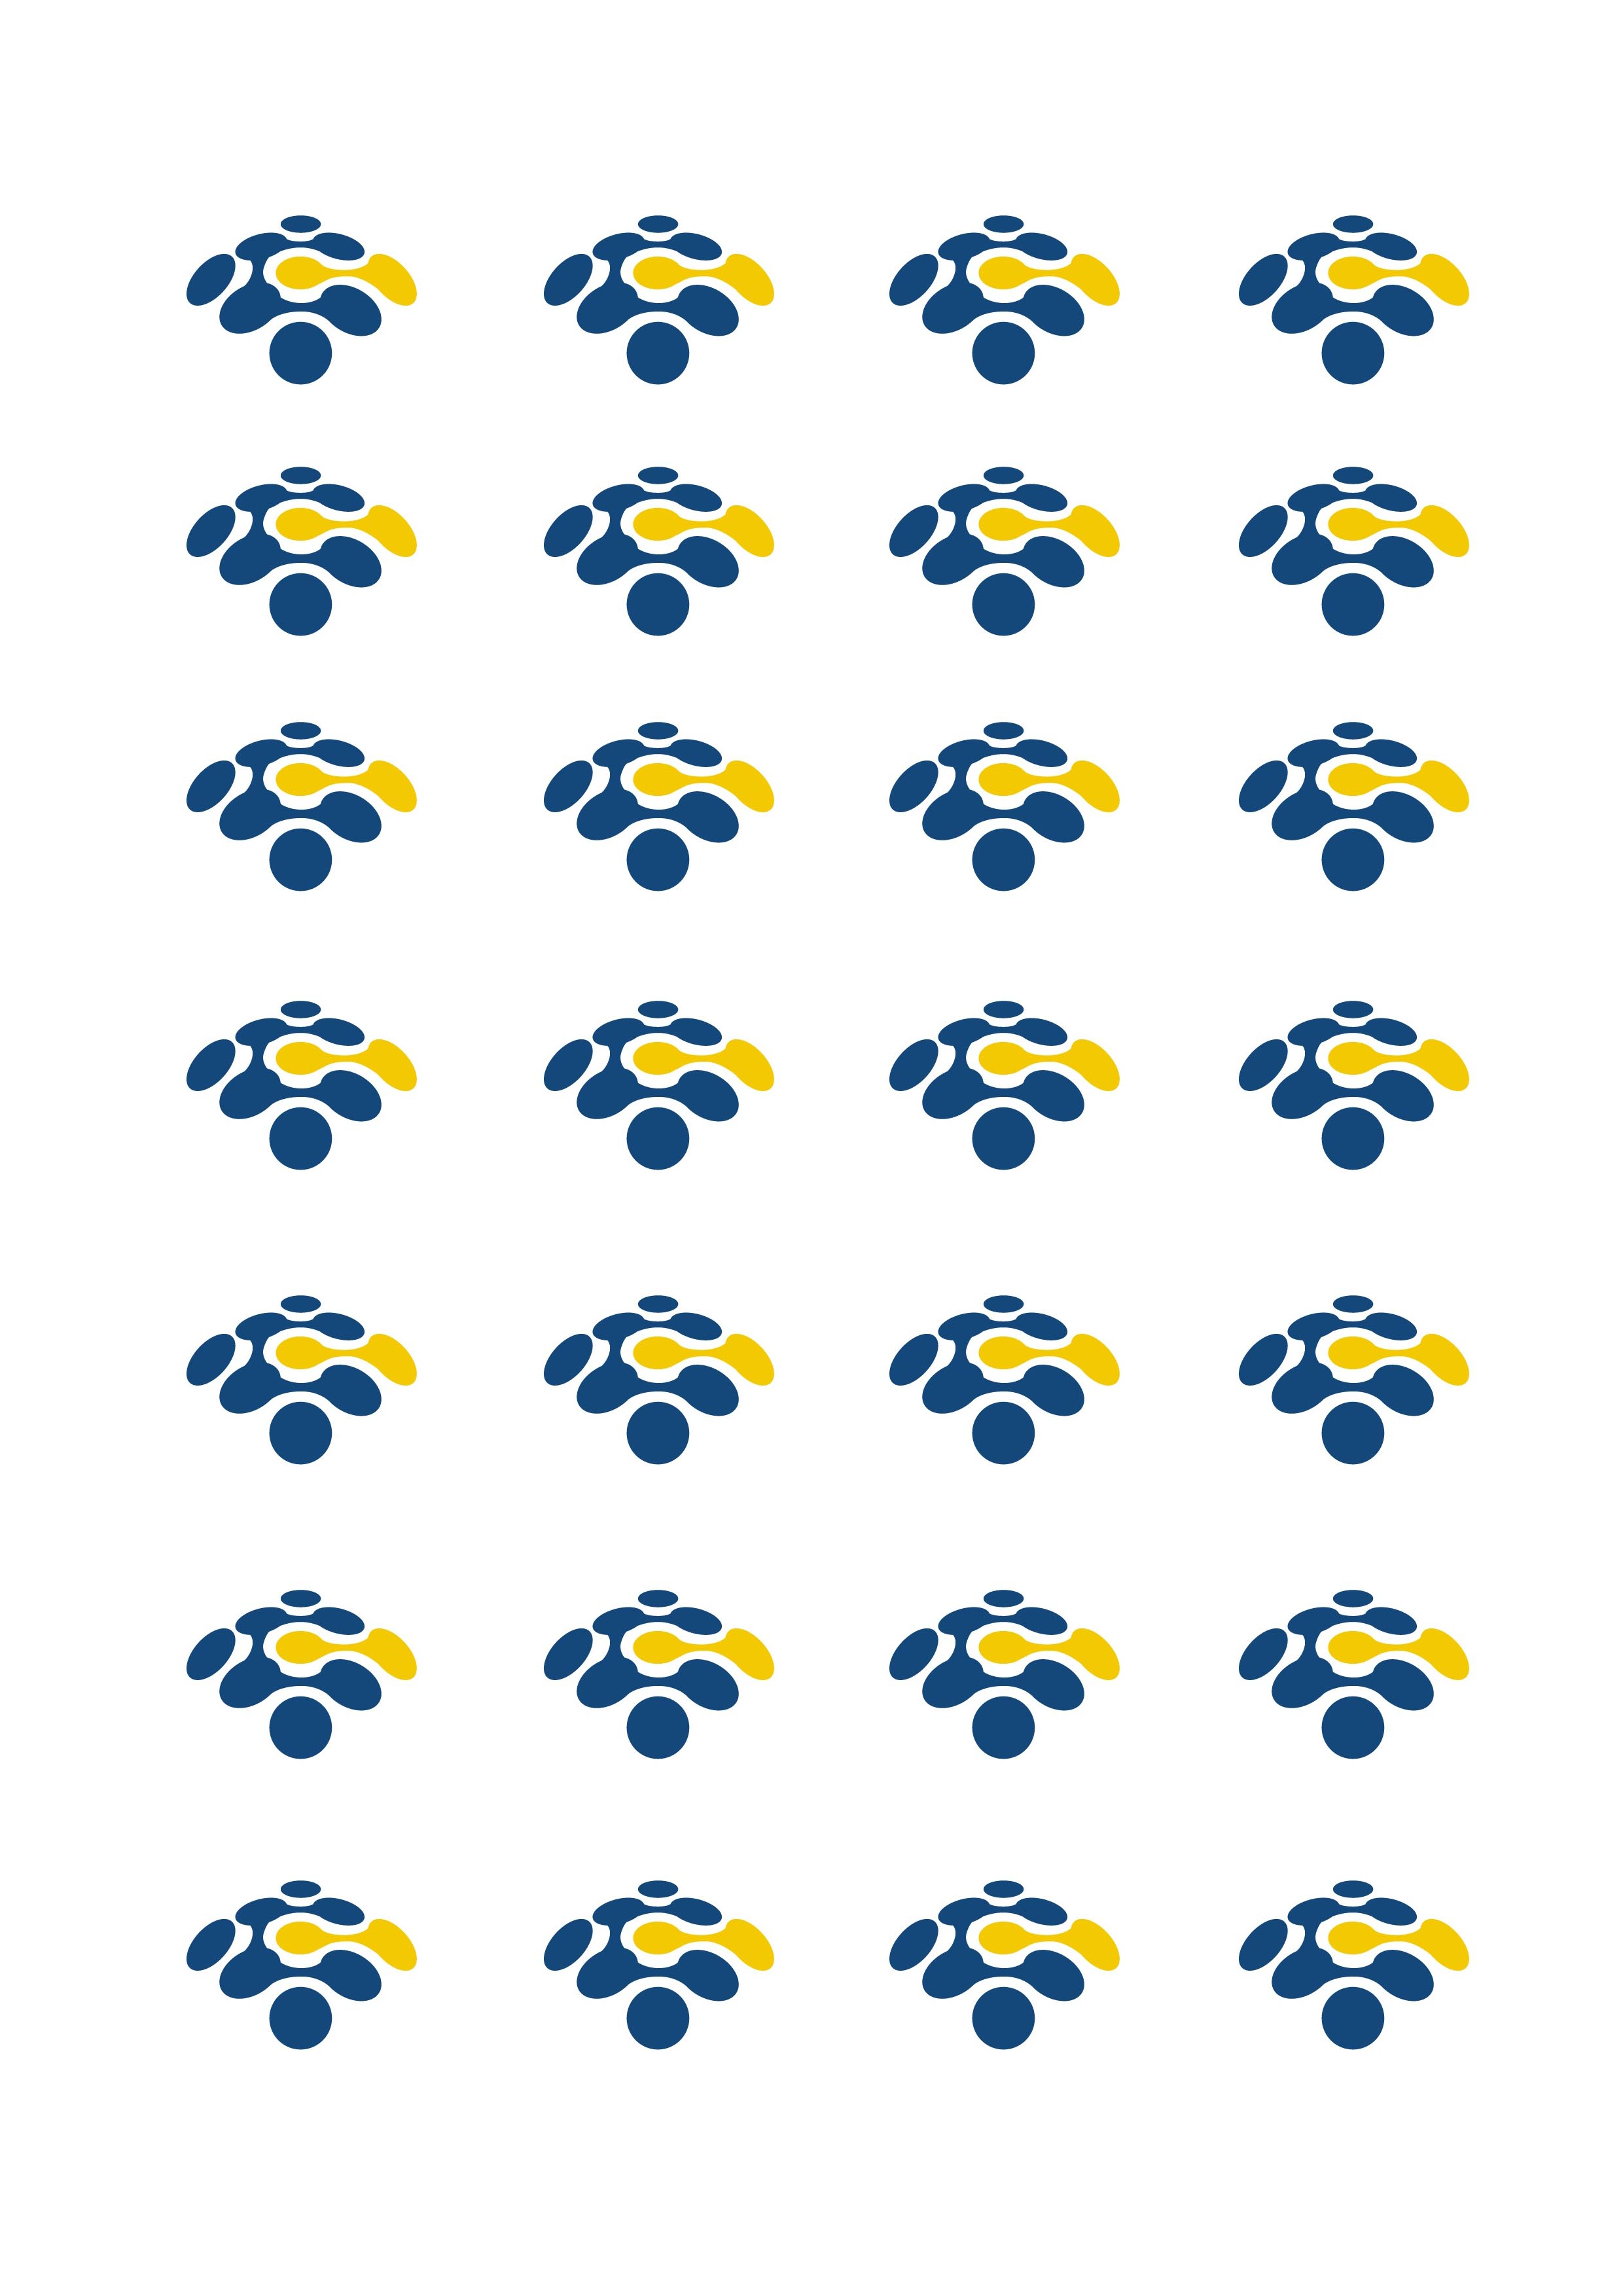
\includegraphics[width=\paperwidth,height=\paperheight]{assets/pens/watermark_pens_a4}%
      };%
    }%
  \fi\fi
}
\newcommand{\AktifkanWatermarkDigilib}{\global\watermarkontrue}
\newcommand{\NonaktifkanWatermarkDigilib}{\global\watermarkonfalse}

% ── Halaman Kosong ───────────────────────────────────────────
% Halaman kosong pada cetak bolak-balik diberi keterangan.
% Mode Digilib: tanpa halaman kosong (cukup \clearpage), karena
% file akan dipotong per bagian untuk berkas yudisium.
\makeatletter
\newif\if@mainmatter
\@mainmatterfalse
\def\cleardoublepage{%
  \clearpage
  \ifdigilib\else
  \if@twoside
  \ifodd\c@page\else
  \hbox{}
  \vspace*{\fill}
  \begin{center}
    \textit{Halaman ini sengaja dikosongkan}
  \end{center}
  \vspace{\fill}
  \if@mainmatter
  \thispagestyle{fancy}  % sudah masuk konten, tampilkan nomor
  \else
  \thispagestyle{empty}  % masih prelim sebelum roman, sembunyikan
  \fi
  \newpage
  \if@twocolumn\hbox{}\newpage\fi
  \fi
  \fi
  \fi
}

% ── Paksa Halaman Ganjil (oneside & twoside) ─────────────────
% \cleartooddpage: lompat ke halaman ganjil berikutnya.
% Jika halaman saat ini sudah ganjil, tidak melakukan apa-apa.
% Jika genap, sisipkan halaman kosong bertuliskan keterangan
% lalu lanjutkan ke halaman ganjil berikutnya.
\newcommand{\cleartooddpage}{%
  \clearpage
  \ifodd\c@page\else
  \hbox{}
  \vspace*{\fill}
  \begin{center}
    \textit{Halaman ini sengaja dikosongkan}
  \end{center}
  \vspace{\fill}
  \thispagestyle{fancy}
  \newpage
  \fi
}
\makeatother
     % base layer: aturan shared
%============================================================
% FORMAT: BUKU PROYEK AKHIR
% Aturan layout khusus Buku PA.
% Di-input SETELAH config/formatting.tex agar bisa override.
%
% Panduan: Buku PA Sarjana Terapan A4 Rev05
%============================================================

% ── Geometri: double-sided, mirror margin Rev05 ───────────────
\geometry{
  a4paper,
  twoside,
  top    = 3cm,
  bottom = 3cm,
  inner  = 4cm,   % Margin sisi jilid (kiri halaman ganjil)
  outer  = 3cm    % Margin luar
}

% ── Spasi Baris ───────────────────────────────────────────────
% \onehalfspacing di sini HANYA berlaku untuk cover, halaman judul,
% dan pengesahan. Mulai halaman prelim, main_buku.tex mengganti
% dengan \setstretch{1.5} (setara visual spasi 1.5 MS Word).
\onehalfspacing

% ── Indentasi Paragraf (Rev05: 1.27cm) ───────────────────────
\setlength{\parindent}{1.27cm}

% ── Override Subsubsection spacing (khusus Buku PA) ──────────
% formatting.tex pakai \titlespacing* (ada bintang) yang men-suppress
% indent paragraf pertama setelah heading. Di Buku PA ini tidak mau —
% paragraf pertama harus tetap mendapat \parindent = 1.27cm agar
% selaras dengan posisi teks subsubsection (yang juga mulai di \parindent).
% Solusi: override dengan \titlespacing TANPA bintang.
\titlespacing{\subsubsection}{\parindent}{3pt}{2pt}

% ── Jarak Atas/Bawah Gambar dan Tabel (khusus Buku PA) ───────
% Base layer (config/formatting.tex) memakai 12pt; Buku PA final
% yang sudah lolos koreksi dosen memakai 15pt.
\setlength{\intextsep}{15pt}
\setlength{\textfloatsep}{15pt}
   % per-dokumen: geometry + spacing

%============================================================
\begin{document}
%============================================================

% ── Halaman Sampul & Judul ───────────────────────────────────
%============================================================
% HALAMAN SAMPUL (Cover Berwarna)
% Dimensi sesuai Panduan Rev05:
%   Logo     : lebar 3,5 cm
%   Header   : tinggi 5 cm (area putih)
%   Garis    : tebal 0,5 cm (warna emas)
%   Konten   : latar belakang biru PENS
%============================================================
\begin{titlepage}
  \newgeometry{top=0pt, bottom=0pt, left=0pt, right=0pt}
  \setlength{\fboxsep}{0pt}
  \pagecolor{pensbiru}

  % ── Bagian 1: Header Putih (tinggi 5 cm) ─────────────────────
  \noindent
  \colorbox{white}{%
    \begin{minipage}[c][5cm][c]{\textwidth}
      \hspace*{3cm}
      \begin{minipage}[c]{4cm}
        \includegraphics[width=3.5cm, keepaspectratio]{assets/pens/logo_pens.png}
      \end{minipage}
      \hfill
      \begin{minipage}[c]{8cm}
        \raggedleft
        {\color{pensbiru}\FontCoverBukuLabel\bfseries PROYEK AKHIR}
      \end{minipage}
      \hspace*{3.5cm}
    \end{minipage}
  }\par\nointerlineskip

  % ── Bagian 2: Garis Emas (tinggi 0,5 cm) ─────────────────────
  \noindent
  \colorbox{penskuning}{%
    \makebox[\textwidth][l]{\rule{0pt}{0.5cm}}%
  }\par\nointerlineskip

  % ── Bagian 3: Konten Biru ─────────────────────────────────────
  \begin{center}
    \color{white}

    \vspace*{1.6cm}

    \begin{minipage}{\dimexpr\paperwidth-6cm\relax}
      \centering
      \FontCoverBukuJudul\bfseries\MakeUppercase{\JudulPA}
    \end{minipage}
    \par

    \vspace{1cm}

    % Identitas mahasiswa: 16pt, bold
    {\FontCoverBukuIsi\bfseries \NamaMahasiswa\par}
    {\FontCoverBukuIsi\bfseries NRP. \NRP\par}

    \vspace{0.8cm}

    % --- Di dalam blok "Dosen Pembimbing" ---
    {\FontCoverBukuIsi\bfseries DOSEN PEMBIMBING\par}
    {\FontCoverBukuIsi \textbf{\NamaPembimbingSatu}\par}
    {\FontCoverBukuIsi \textbf{NIP. \NIPPembimbingSatu}\par}
    \vspace{0.5cm}
    {\FontCoverBukuIsi \textbf{\NamaPembimbingDua}\par}
    {\FontCoverBukuIsi \textbf{NIP. \NIPPembimbingDua}\par}

    % Logika Pembimbing ke-3 (Akademik)
    \ifcsvoid{NamaPembimbingTiga}{}{%
      \vspace{0.3cm}
      {\FontCoverBukuIsi \textbf{\NamaPembimbingTiga}\par}
      {\FontCoverBukuIsi \textbf{NIP. \NIPPembimbingTiga}\par}
    }

    % Logika Pembimbing Industri/Dosen Tambahan
    \ifcsvoid{NamaPembimbingIndustri}{}{%
      \vspace{0.8cm}
      {\FontCoverBukuIsi\bfseries PEMBIMBING INDUSTRI\par}
      {\FontCoverBukuIsi \textbf{\NamaPembimbingIndustri}\par}
      \ifcsvoid{NIPPembimbingIndustri}{}{%
        {\FontCoverBukuIsi \textbf{NIP. \NIPPembimbingIndustri}\par}
      }
      \ifcsvoid{NamaPerusahaanIndustri}{}{%
        {\FontCoverBukuIsi \textbf{\NamaPerusahaanIndustri}\par}
      }

    }

    \vspace{1cm}

    % Program studi: 16pt, bold, kapital
    {\FontCoverBukuIsi\bfseries PROGRAM STUDI SARJANA TERAPAN\par}
    {\FontCoverBukuIsi\bfseries \MakeUppercase{\NamaProdi}\par}
    {\FontCoverBukuIsi\bfseries \MakeUppercase{\NamaDepartemen}\par}

    \vspace{0.5cm}

    % Institusi dan tahun: 16pt, bold, kapital
    {\FontCoverBukuIsi\bfseries POLITEKNIK ELEKTRONIKA NEGERI SURABAYA\par}
    {\FontCoverBukuIsi\bfseries \TahunLulus\par}

  \end{center}

  \restoregeometry
\end{titlepage}
\pagecolor{white}
%============================================================
% HALAMAN JUDUL DALAM
% Sama dengan cover tetapi tanpa warna (hitam-putih).
% "PROYEK AKHIR" rata kanan, sisanya rata tengah.
%============================================================
\newpage
\thispagestyle{empty}
\addtocontents{toc}{\protect\cftpagenumbersoff{chapter}}
\addcontentsline{toc}{chapter}{HALAMAN JUDUL}
\addtocontents{toc}{\protect\cftpagenumberson{chapter}}

% "PROYEK AKHIR" rata kanan
\begin{flushright}
  {\FontJudulDalamLabel\bfseries PROYEK AKHIR\par}
\end{flushright}

\vspace{1.5cm}

\begin{center}

  \begin{minipage}{1\textwidth}
    \centering
    \FontJudulDalamJudul\bfseries\MakeUppercase{\JudulPA}
  \end{minipage}
  \par

  \vspace{1.2cm}

  % Identitas mahasiswa: 16pt, bold
  {\FontJudulDalamIsi\bfseries \NamaMahasiswa\par}
  {\FontJudulDalamIsi\bfseries NRP. \NRP\par}

  \vspace{0.8cm}

  % --- Di dalam blok "Dosen Pembimbing" ---
  {\FontJudulDalamIsi\bfseries DOSEN PEMBIMBING\par}
  {\FontJudulDalamIsi \NamaPembimbingSatu\par}
  {\FontJudulDalamIsi NIP. \NIPPembimbingSatu\par}
  \vspace{0.5cm}
  {\FontJudulDalamIsi \NamaPembimbingDua\par}
  {\FontJudulDalamIsi NIP. \NIPPembimbingDua\par}

  % Logika Pembimbing ke-3 (Akademik)
  \ifcsvoid{NamaPembimbingTiga}{}{%
    \vspace{0.3cm}
    {\FontJudulDalamIsi \NamaPembimbingTiga\par}
    {\FontJudulDalamIsi NIP. \NIPPembimbingTiga\par}
  }

  % Logika Pembimbing Industri
  \ifcsvoid{NamaPembimbingIndustri}{}{%
    \vspace{0.8cm}
    {\FontJudulDalamIsi\bfseries PEMBIMBING INDUSTRI\par}
    {\FontJudulDalamIsi \NamaPembimbingIndustri\par}
    \ifcsvoid{NamaPerusahaanIndustri}{}{%
      {\FontJudulDalamIsi \NamaPerusahaanIndustri\par}
    }
  }

  \vspace{1cm}

  % Program studi: 16pt, bold, kapital
  {\FontJudulDalamIsi\bfseries PROGRAM STUDI SARJANA TERAPAN\par}
  {\FontJudulDalamIsi\bfseries \MakeUppercase{\NamaProdi}\par}
  {\FontJudulDalamIsi\bfseries \MakeUppercase{\NamaDepartemen}\par}

  \vspace{0.5cm}

  % Institusi dan tahun: 16pt, bold, kapital
  {\FontJudulDalamIsi\bfseries POLITEKNIK ELEKTRONIKA NEGERI SURABAYA\par}
  {\FontJudulDalamIsi\bfseries \TahunLulus\par}

\end{center}
%============================================================
% HALAMAN PENGESAHAN
% Watermark background otomatis untuk 1 atau lebih halaman.
%============================================================
\cleardoublepage
\pagestyle{empty} % Memastikan seluruh halaman pengesahan tanpa nomor/header
\addtocontents{toc}{\protect\cftpagenumbersoff{chapter}}
\addcontentsline{toc}{chapter}{HALAMAN {PENGESAHAN}}
\addtocontents{toc}{\protect\cftpagenumberson{chapter}}

\ifpengesahanpdf
% Sisipkan lembar pengesahan PDF yang sudah ditandatangani
% (aktifkan \pengesahanpdftrue di main_buku.tex / config/toggles.tex)
\includepdf[pages=-]{\FilePengesahanPDF}
\else

% 1. Nyalakan watermark secara otomatis mulai dari halaman ini
\AddToShipoutPictureBG{%
  \tikz[remember picture, overlay]
  \node[inner sep=0pt] at (current page.center){%
    \includegraphics[width=\paperwidth, height=\paperheight]{assets/pens/background_pens_repeated.png}%
  };
}

\begin{center}
  {\FontPengesahanLabel\bfseries HALAMAN PENGESAHAN\par}
  \vspace{0.8cm}

  \begin{minipage}{1\textwidth}
    \centering
    \FontPengesahanJudul\bfseries\MakeUppercase{\JudulPA}
  \end{minipage}
  \par

  \vspace{0.6cm}

  {\FontPengesahanIsi Oleh:\par}
  \vspace{0.1cm}

  {\FontPengesahanIsi\bfseries
    \NamaMahasiswa\par
  NRP. \NRP\par}

  \vspace{0.6cm}

  \begin{spacing}{1}
    {\FontPengesahanIsi\bfseries
      Proyek Akhir ini digunakan sebagai salah satu syarat untuk\\
      memperoleh Gelar \GelarLulus\\
      di Politeknik Elektronika Negeri Surabaya\\
    \TahunLulus\par}
  \end{spacing}
\end{center}

\vspace{0.2cm}
\begin{center}
  {\FontPengesahanIsi\bfseries Disetujui oleh:}
\end{center}
\vspace{0.2cm}

% Daftar pembimbing dan penguji beserta kolom tanda tangan
\noindent
{\FontPengesahanIsi
  \begin{tabular}{@{}l c l c@{}}
    Pembimbing 1 & : & \NamaPembimbingSatu   & (\hspace{2.5cm}) \\
    &   & NIP. \NIPPembimbingSatu & \\[3pt]
    Pembimbing 2 & : & \NamaPembimbingDua   & (\hspace{2.5cm}) \\
    &   & NIP. \NIPPembimbingDua & \\[3pt]

    % Baris kondisional Pembimbing 3 (Akademik)
    \ifcsvoid{NamaPembimbingTiga}{}{%
      Pembimbing 3 & : & \NamaPembimbingTiga   & (\hspace{2.5cm}) \\
      &   & NIP. \NIPPembimbingTiga & \\[3pt]
    }

    % Baris kondisional Pembimbing Industri
    \ifcsvoid{NamaPembimbingIndustri}{}{%
      Pembimbing Industri & : & \NamaPembimbingIndustri & (\hspace{2.5cm}) \\
      &   &                        & \\[3pt]
    }

    Penguji 1    & : & \NamaPengujiSatu     & (\hspace{2.5cm}) \\
    &   & NIP. \NIPPengujiSatu   & \\[3pt]
    Penguji 2    & : & \NamaPengujiDua      & (\hspace{2.5cm}) \\
    &   & NIP. \NIPPengujiDua    & \\
  \end{tabular}
}

\vspace{0.3cm}

% 2. Blok Mengetahui dibungkus dalam minipage
%    Jika ruang tidak cukup, SELURUH kotak ini akan pindah ke halaman 2.
\noindent
\begin{minipage}{\textwidth}
  \begin{center}
    {\FontPengesahanIsi\bfseries Mengetahui,}\par
    {\FontPengesahanIsi
      Ketua Program Studi Sarjana Terapan \NamaProdi\par
    Politeknik Elektronika Negeri Surabaya}\par
    \vspace{1.5cm}
    {\FontPengesahanIsi
      \underline{\NamaKetuaProdi}\par
    NIP. \NIPKetuaProdi\par}
  \end{center}
\end{minipage}

% 3. Paksa render halaman terakhir, lalu MATIKAN watermark agar tidak bocor
\clearpage
\ClearShipoutPictureBG
\fi

% ── Spasi Baris 1.5 (mulai halaman prelim sampai akhir) ───────
% Cover, halaman judul, dan pengesahan di atas memakai \onehalfspacing
% (diset di formats/format_buku.tex). Mulai dari sini dipakai
% \setstretch{1.5}, karena \onehalfspacing LaTeX (±18pt per baris)
% jauh lebih rapat dari spasi 1.5 MS Word (±20.7pt).
% \setstretch{1.5} menghasilkan ±21.75pt (sama dengan Buku PA final
% yang sudah lolos koreksi dosen).
\setstretch{1.5}

% ── Halaman Prelim (penomoran romawi kecil) ──────────────────
\cleardoublepage
\pagestyle{fancy}
\pagenumbering{roman}
\setcounter{page}{1}
\makeatletter\@mainmattertrue\makeatother
%============================================================
% HALAMAN PERNYATAAN ORISINALITAS  (halaman i)
%============================================================
\addcontentsline{toc}{chapter}{PERNYATAAN ORISINALITAS}
\thispagestyle{fancy}

\begin{center}
  {\FontPernyataanLabel\bfseries PERNYATAAN ORISINALITAS\par}
\end{center}
\vspace{1.5cm}

{\FontPernyataanIsi
  \begin{spacing}{1.5}

    \noindent Dengan ini saya menyatakan bahwa bagian atau keseluruhan proyek akhir ini:

    \begin{enumerate}[label=\arabic*., leftmargin=*]
      \item Adalah hasil karya sendiri dan tidak mengandung unsur plagiat dari pihak lain,
      \item Tidak pernah diajukan untuk mendapatkan gelar akademis pada suatu Perguruan Tinggi,
      \item Tidak pernah dipublikasikan atau ditulis oleh pihak lain,
      \item Mencantumkan rujukan dan kutipan dengan jujur dan benar terhadap sumber referensi
        lain yang menunjang pembahasan pada proyek akhir ini.
    \end{enumerate}

    Apabila ditemukan bukti bahwa pernyataan saya di atas tidak benar, maka saya bersedia
    menerima sanksi sesuai dengan ketentuan yang berlaku di Politeknik Elektronika Negeri
    Surabaya.

  \end{spacing}

  \vspace{2.5cm}

  % Blok tanggal dan tanda tangan di sebelah kanan
  \hfill
  \begin{minipage}{6.5cm}
    \TanggalSidang\\[2cm]
    \underline{\bfseries \NamaMahasiswa}\\
    \bfseries NRP. \NRP
  \end{minipage}
}
%============================================================
% HALAMAN PERNYATAAN PENGALIHAN HAK CIPTA  (halaman ii)
%============================================================
\cleardoublepage
\addcontentsline{toc}{chapter}{PERNYATAAN PENGALIHAN HAK CIPTA}
\thispagestyle{fancy}

\ifhakciptapdf
% Sisipkan PDF pernyataan yang sudah ditandatangani di atas materai
% (aktifkan \hakciptapdftrue di config/toggles.tex)
\includepdf[pages=-, pagecommand={\thispagestyle{fancy}}]{\FileHakCiptaPDF}
\else

\begin{center}
  {\FontPernyataanLabel\bfseries PERNYATAAN PENGALIHAN HAK CIPTA\par}
\end{center}
\vspace{1.5cm}

\noindent Dengan ini, saya yang bertanda tangan di bawah ini:

\vspace{0.5cm}
\noindent
\begin{tabular}{@{}ll p{10cm} @{}}
  Nama              & : & \NamaMahasiswa \\
  NRP               & : & \NRP \\
  Judul Proyek Akhir & : & \JudulPA \\
  Tanggal           & : & \TanggalSidang \\
\end{tabular}
\vspace{0.5cm}

\noindent menyatakan bahwa saya selaku penulis (dan/atau mewakili seluruh penulis) secara
sadar dan sukarela mengalihkan hak cipta (\textit{copyright}) atas proyek akhir tersebut
kepada Politeknik Elektronika Negeri Surabaya.

\noindent Demikian pernyataan ini saya buat dengan sebenar-benarnya dan tanpa paksaan
dari pihak mana pun.

\vspace{2cm}
\begin{flushleft}
  Hormat saya,\\[1cm]

  % Ruang kosong untuk materai & tanda tangan (tempel setelah dicetak)
  \vspace{2cm}

  \underline{\bfseries \NamaMahasiswa}
\end{flushleft}
\fi

% Mode Digilib: watermark aktif mulai Abstrak (tidak berefek jika \digilibfalse)
\cleardoublepage
\AktifkanWatermarkDigilib

%============================================================
% HALAMAN ABSTRAK  (halaman iii)
% Tulis abstrak dalam Bahasa Indonesia, 300-500 kata.
% Isi: latar belakang (~1 kalimat), permasalahan (1-2 kalimat),
%      solusi (~5 kalimat), kinerja (~2 kalimat).
%============================================================
\cleardoublepage
\chapter*{ABSTRAK}
\addcontentsline{toc}{chapter}{ABSTRAK}
\thispagestyle{fancy}

Abstrak adalah versi ringkas dari proyek akhir yang dituliskan dengan sistematis.
Abstrak seharusnya memberikan gambaran ringkas dari konten-konten yang penting dari
proyek akhir. Kata-kata yang ada pada abstrak seharusnya dipilih dengan cermat dan
disusun dengan jelas untuk mendeskripsikan isi proyek akhir. Abstrak memuat pembahasan
berikut: Latar belakang permasalahan (sekitar 1 kalimat), Permasalahan (1-2 kalimat),
Solusi yang ditawarkan (sekitar 5 kalimat), dan Kinerja (sekitar 2 kalimat). Latar
belakang permasalahan diambil dari \textit{problem domain} pada penelitian proyek akhir.
Permasalahan menjelaskan tingkat urgensi dari \textit{problem} pada penelitian proyek
akhir. Solusi mendiskusikan tujuan utama pada proyek akhir, klaim orisinalitas
penelitian, skala penelitian, dan mendiskusikan metodologi penyelesaian masalah. Kinerja
membahas ringkasan eksperimen, hasil ujicoba dan analisis kinerja. Abstrak ditulis dalam
300-500 kata.

\vspace{0.5cm}
\noindent\textbf{Kata Kunci}

\noindent kata1, kata2, kata3, kata4, kata5
%============================================================
% HALAMAN ABSTRACT  (halaman iv)
% Terjemahan abstrak ke dalam Bahasa Inggris, ditulis miring.
% Isi sama dengan abstrak.tex: 300-500 kata.
%============================================================
\cleardoublepage
\chapter*{ABSTRACT}
\addcontentsline{toc}{chapter}{ABSTRACT}
\thispagestyle{fancy}

\textit{The abstract is written in English as a translation of the Indonesian abstract
  above. It should be written in italic format and contain the same structure: background
  (approx.\ 1 sentence), problem statement (1--2 sentences), proposed solution (approx.\
  5 sentences), and performance evaluation (approx.\ 2 sentences). The abstract should be
300--500 words.}

\vspace{0.5cm}
\noindent\textbf{Keywords}

\noindent keyword1, keyword2, keyword3, keyword4, keyword5
%============================================================
% HALAMAN KATA PENGANTAR  (halaman v)
% Gunakan bahasa formal. Sertakan ucapan terima kasih kepada
% pihak-pihak yang berkontribusi pada proyek akhir.
%============================================================
\cleardoublepage
\chapter*{KATA PENGANTAR}
\addcontentsline{toc}{chapter}{KATA PENGANTAR}
\thispagestyle{fancy}

Penulis dapat memberikan kata pengantar sebagai prakata dalam mengawali penulisan buku
proyek akhir. Penulis dapat menyampaikan cerita-cerita dan kesan saat melakukan
penelitian sampai penulisan buku proyek akhir, memberikan apresiasi dan ucapan terima
kasih kepada pihak-pihak yang telah membantu penulis dalam penelitian dan penulisan buku
proyek akhir, ataupun memberikan motivasi dan pesan kepada pembaca. Kata pengantar
seharusnya menggunakan kata-kata yang baik dan gaya bahasa formal. Pada bagian kata
pengantar dapat ditambahkan ucapan terima kasih kepada pihak-pihak yang berkontribusi
dalam pelaksanaan proyek akhir.

% ── Daftar Isi, Gambar, Tabel ────────────────────────────────
\cleardoublepage
\tableofcontents

\cleardoublepage
\begingroup
\renewcommand*{\addvspace}[1]{}
\listoffigures
\endgroup
\addcontentsline{toc}{chapter}{DAFTAR GAMBAR}

\cleardoublepage
\begingroup
\renewcommand*{\addvspace}[1]{}
\listoftables
\endgroup
\addcontentsline{toc}{chapter}{DAFTAR TABEL}

% ── Isi Utama (penomoran Arab dimulai dari 1) ─────────────────
\cleardoublepage
\pagenumbering{arabic}
\setcounter{page}{1}

% Tentukan file sistematika sesuai jenis dokumen ini
\newcommand{\SistematikaFile}{pages/sistematika_5bab}
%============================================================
% BAB 1: PENDAHULUAN
% Struktur:
%   Proposal/Progres (\ifbukupa = false):
%     1.1 Latar Belakang, 1.2 Permasalahan, 1.3 Tujuan,
%     1.4 Manfaat, 1.5 Sistematika Penulisan
%   Buku PA (\ifbukupa = true):
%     1.1 Latar Belakang, 1.2 Permasalahan, 1.3 Batasan Masalah,
%     1.4 Tujuan, 1.5 Manfaat, 1.6 Sistematika Penulisan
%============================================================
\chapter{PENDAHULUAN}

\section{LATAR BELAKANG}

Deskripsikan latar belakang dari permasalahan yang akan diangkat pada penelitian proyek
akhir. Latar belakang berisi penjelasan dari \textit{Problem Domain} yang termuat pada
judul penelitian. Misalkan penulis mengambil suatu judul ``Deteksi Penyakit Kanker
Dengan Sistem Pakar Berbasis Fuzzy'', maka \textit{Problem Domain}-nya adalah tentang
penyakit kanker, sehingga penulis dapat menceritakan tingkat urgensinya seperti
kenaikan jumlah penderita dari tahun ke tahun. Latar belakang yang baik berisikan
\textit{problem domain} yang mempunyai tingkat urgensi tinggi.

% Contoh kutipan tidak langsung (parafrase):
% Menurut penelitian sebelumnya, hal ini sangat penting dilakukan \cite{}.

\section{PERMASALAHAN}

Deskripsikan dengan jelas permasalahan yang ingin diteliti pada proyek akhir.
Permasalahan berisi penjelasan dari \textit{Problem} yang termuat pada judul penelitian.
Deskripsi masalah sebaiknya dituliskan dengan gaya bahasa deskriptif. Uraian
permasalahan yang baik manakala penulis berhasil meyakinkan pembaca tentang seberapa
tinggi tingkat urgensi dari permasalahan tersebut, sehingga pembaca yakin bahwa
permasalahan tersebut membutuhkan solusi dari penelitian proyek akhir.

% Batasan Masalah: hanya tampil di Buku PA
\ifbukupa
\section{BATASAN MASALAH}

Deskripsikan dengan jelas hal-hal yang perlu dibatasi dari permasalahan yang diselesaikan
dalam proyek akhir. Deskripsi batasan masalah sebaiknya dituliskan dalam bentuk
\textit{itemik}.

\begin{enumerate}[label=\arabic*., leftmargin=*]
  \item Batasan masalah pertama.
  \item Batasan masalah kedua.
  \item Batasan masalah ketiga.
\end{enumerate}
\fi

\section{TUJUAN}

Deskripsikan dengan jelas tujuan penelitian proyek akhir yang diangkat. Tujuan proyek
akhir harus jelas, singkat, dan mengandung klaim orisinalitas. Tuliskan secara
argumentatif apa saja fitur-fitur yang ditawarkan pada penelitian sebagai solusi baru
untuk mengklaim orisinalitas. Tujuan sebaiknya diawali dengan kalimat pembuka seperti:

``Penelitian proyek akhir ini mengajukan suatu pendekatan baru untuk \ldots dengan
mempresentasikan \ldots''. Kalimat-kalimat selanjutnya kemudian memperjelas
fitur-fitur unik yang ditawarkan pada penelitian sebagai suatu solusi untuk menjawab
permasalahan.

\section{MANFAAT}

Uraikan kontribusi proyek akhir pada pengembangan ilmu pengetahuan teknologi dan seni,
pemecahan masalah pembangunan, atau pengembangan kelembagaan. Kontribusi sebaiknya
bersifat spesifik, tidak terlalu luas, dan tidak terkesan mengada-ada. Jelaskan siapa
yang mendapatkan manfaat dari penelitian dan dalam bentuk apa manfaatnya.

\section{SISTEMATIKA PENULISAN}

Jelaskan tentang sistematika pembahasan dalam buku proyek akhir yang meliputi:

% File sistematika ditentukan oleh runner (main_*.tex) via \SistematikaFile.
% Proposal: pages/sistematika_3bab | Progres/Buku: pages/sistematika_5bab
\input{\SistematikaFile}

%============================================================
% BAB 2: KAJIAN PUSTAKA
%============================================================
\chapter{KAJIAN PUSTAKA}

Awali pembahasan pada bab ini dengan mengutarakan \textit{Problem} pada
\textit{Problem Domain} dari proyek akhir. Setelah itu, penjelasan tersebut diiringi
dengan teori-teori penunjang pada bidang pengetahuan yang terkait dengan
\textit{Problem Domain} dan \textit{Problem}. Untuk lebih menguatkan klaim orisinalitas
proyek akhir, perlu diberikan ulasan tentang penelitian-penelitian terkait yang juga
bertujuan menyelesaikan \textit{Problem} tersebut.

\section{DESKRIPSI PERMASALAHAN}

Deskripsikan dengan jelas dan detail dari permasalahan yang ingin diselesaikan pada
proyek akhir. Permasalahan berisi penjelasan dari \textit{Problem} yang termuat pada
judul kegiatan. Deskripsi masalah sebaiknya dituliskan dengan gaya bahasa deskriptif.
Deskripsi masalah boleh memuat gambar, tabel, dan skema tertentu untuk mengilustrasikan
permasalahan.

\section{TEORI PENUNJANG}

Uraikan dengan jelas dasar teori yang menunjang penelitian proyek akhir. Teori penunjang
menguraikan dasar-dasar teori, temuan, dan bahan dari pustaka ilmiah lain yang dijadikan
landasan untuk melakukan proyek akhir yang diusulkan. Uraian dalam Teori Penunjang
menjadi landasan untuk menyusun kerangka atau konsep yang akan digunakan dalam proyek
akhir. Jangan lupa untuk menyebutkan semua kutipan dengan rujukan yang jelas seperti
ini \cite{buku_contoh}.

\subsection{Sub-Teori Pertama}

Uraikan sub-teori pertama di sini.

\subsection{Sub-Teori Kedua}

Uraikan sub-teori kedua di sini.

\section{PENELITIAN TERKAIT}

Penelitian terkait memuat hasil penelitian pihak lain yang mempunyai \textit{Problem}
yang sama dengan penelitian kita, tetapi dengan menggunakan \textit{Uniqueness} yang
berbeda. Ceritakan bagaimana penelitian-penelitian terkait telah mencoba menyelesaikan
permasalahan yang sama, dengan cara mereka masing-masing, yang ditunjukkan dengan
kutipan terhadap pustaka. Penelitian terkait yang baik melibatkan kajian pustaka yang
relevan dan terpercaya dari jurnal ilmiah internasional ataupun nasional, presentasi
ilmiah internasional ataupun nasional, dan buku atau catatan rujukan ilmiah. Penulis
harus mencantumkan sumber referensi pada daftar pustaka manakala melakukan rujukan dan
kutipan dari pihak lain secara jujur dan benar seperti ini \cite{jurnal_contoh}.
Pencantuman sumber referensi perlu dilakukan baik terhadap kutipan langsung ataupun
kutipan tidak langsung (parafrase).

Untuk kutipan langsung dan pendek (1--2 baris), cara penulisan rujukan dilakukan dengan
memberikan tanda petik ganda di awal dan akhir kutipan, ditulis miring, kemudian diiringi
sumber referensi, seperti ini \textit{``Ini contoh penulisan rujukan untuk kutipan
langsung dan pendek''}\cite{buku_contoh,jurnal_contoh}. Sedangkan untuk kutipan langsung
dan panjang (lebih dari 2 baris), penulis dapat menuliskannya seperti di bawah ini.

\begin{kutipanpanjang}
  ``Ini contoh penulisan rujukan untuk kutipan langsung dan panjang, ditulis pada
  paragraf terpisah dengan memberikan tanda petik ganda di awal dan akhir kutipan,
  ukuran font 10 point dan margin kanan kiri yang masuk 10 mm dari batas penulisan,
  kemudian diiringi dengan sumber referensi pada daftar pustaka.'' \cite{buku_contoh}
\end{kutipanpanjang}

Untuk kutipan tidak langsung (parafrase), penulis dapat menuliskan sumber referensi
setelah kalimat parafrase selesai, seperti ini \cite{online_contoh}.
%============================================================
% BAB 3: DESAIN SISTEM
%============================================================
\chapter{DESAIN SISTEM}

Uraian pada bab ini meliputi model yang digunakan, rancangan proyek akhir, variabel
dalam proyek akhir, teknik pengumpulan data, dan analisis data. Awali pembahasan pada
bab ini dengan penjelasan umum tentang solusi yang ditawarkan untuk menjawab
\textit{Problem}.

\section{DESKRIPSI SOLUSI}

Deskripsikan solusi yang ditawarkan pada buku proyek akhir dengan jelas dan detail.
Tuliskan secara argumentatif apa saja fitur-fitur yang ditawarkan sebagai solusi baru.
Terangkan secara argumentatif tentang fitur-fitur unik pemodelan yang ditawarkan
sehingga dapat digunakan untuk menyelesaikan permasalahan.

\section{PERANCANGAN SISTEM}

Desain sistem adalah penjelasan teknikal dari solusi yang berisi urutan-urutan proses
yang akan dilakukan untuk menyelesaikan masalah. Akan lebih mudah dicerna apabila
penjelasan ini disertai dengan diagram sistem secara \textit{high-level view} sehingga
pembaca mendapatkan gambaran menyeluruh tentang desain sistem. Gambar~\ref{fig:desain_sistem}
menunjukkan bagan desain sistem yang mempunyai tiga bagian.

% ── Contoh gambar desain sistem ──────────────────────────────
\begin{figure}[H]
  \centering
  \includegraphics[width=0.6\textwidth]{assets/gambar_desain_sistem.jpeg}
  \caption{Desain sistem dari solusi yang ditawarkan}
  \label{fig:desain_sistem}
\end{figure}

% ── Contoh gambar dengan sumber kutipan ──────────────────────
% Sumber dicantumkan di bawah gambar, di atas caption, ukuran 11pt
\begin{figure}[H]
  \centering
  \includegraphics[width=0.6\textwidth]{assets/gambar_kutipan.png}

  \vspace{4pt}
  {\FontSumber\itshape Sumber: http://alamat-sumber.com/gambar.jpg\par}

  \caption{Contoh gambar kutipan}
  \label{fig:gambar_kutipan}
\end{figure}

\subsection{Bagian 1}

Disini penulis dapat menjelaskan lebih terperinci apa saja yang ada pada bagian
ini. Jika bagian ini mempunyai sub bagian yang perlu diperjelas dalam
pembahasan, penulis dapat menuliskannya dalam sub pembahasan pada bagian ini.

\subsubsection{Aaaa}

Disini penulis dapat membahas sub bagian Aaaa lebih terperinci. Deskripsi
pembahasan seharusnya singkat, padat dan jelas, sehingga membuat pembaca
memahami maksud penulis yang tertuang dalam tulisan. Apabila pembahasan penulis
memerlukan penulisan persamaan matematis, penulis dapat menuliskannya seperti
pada Persamaan~\ref{eq:binomial}.

\begin{equation}
  (x+a)^n = \sum_{k=0}^{n} \binom{n}{k} x^k a^{n-k}
  \label{eq:binomial}
\end{equation}

Persamaan~\ref{eq:binomial} menunjukkan teorema binomial yang merupakan dasar dari
metode yang digunakan.

% ── Contoh tabel dengan sumber kutipan (tabularray) ──────────
\begin{table}[H]
  \centering
  \caption{Contoh penulisan tabel otomatis}
  \label{tab:contoh1}
  \begin{tblr}{colspec={c c c}}
    Kolom 1  & Kolom 2  & Kolom 3  \\
    Data 1-1 & Data 1-2 & Data 1-3 \\
    Data 2-1 & Data 2-2 & Data 2-3 \\
  \end{tblr}

  \vspace{4pt}
  {\FontSumber Sumber: Badan Pusat Pengolahan Data, 2026 \cite{buku_contoh}\par}
\end{table}

\subsection{Bagian 2}

Disini penulis dapat menjelaskan lebih terperinci apa saja yang ada pada Bagian 2 ini.
Deskripsi pembahasan seharusnya singkat, padat, dan jelas sehingga membuat pembaca
memahami maksud penulis yang tertuang dalam tulisan.

% ── Contoh tabel biasa tanpa sumber (tabularray) ─────────────
\begin{table}[H]
  \centering
  \caption{Contoh penulisan tabel 2}
  \label{tab:contoh2}
  \begin{tblr}{colspec={c c c c}}
    Kolom 1 & Kolom 2 & Kolom 3 & Kolom 4 \\
    Data 1-1 & Data 1-2 & Data 1-3 & Data 1-4 \\
    Data 2-1 & Data 2-2 & Data 2-3 & Data 2-4 \\
  \end{tblr}
\end{table}

\begin{equation}
  F = m \cdot a
  \label{eq:newton}
\end{equation}

\subsection{Bagian 3}

Disini penulis dapat menjelaskan lebih terperinci apa saja yang ada pada Bagian 3 ini.
Deskripsi pembahasan seharusnya singkat, padat, dan jelas sehingga membuat pembaca
memahami maksud penulis yang tertuang dalam tulisan.

\subsubsection{Aaa}

aaa

\subsection{Bagian 4}

bbb

\subsubsection{Bbbb}

bbbb

\begin{equation}
  \lim_{x \to c} f(x) = L
  \label{eq:limit}
\end{equation}
%============================================================
% BAB 4: EKSPERIMEN DAN ANALISIS
%============================================================
\chapter{EKSPERIMEN DAN ANALISIS}

Uraian pada bab ini meliputi parameter eksperimen, karakteristik data, skenario
ujicoba, tempat dan waktu eksperimen, spesifikasi peralatan ujicoba, cara penafsiran
dan penyimpulan hasil proyek akhir. Untuk proyek akhir yang menggunakan metode
kualitatif, dapat dijelaskan pendekatan yang digunakan, proses pengumpulan dan analisis
informasi, proses penafsiran, dan penyimpulan hasil proyek akhir. Analisis hasil
eksperimen seharusnya dihubungkan kembali dengan permasalahan.

\section{PARAMETER EKSPERIMEN}

Disini penulis dapat membahas parameter eksperimen lebih terperinci. Deskripsi
pembahasan seharusnya singkat, padat, dan jelas sehingga membuat pembaca memahami
maksud penulis yang tertuang dalam tulisan. Dalam eksperimen ini menggunakan persamaan
sebagai berikut:

\begin{equation}
  y = mx + c
  \label{eq:linear}
\end{equation}
\begin{equation}
  \frac{y - y_1}{x - x_1} = \frac{y_2 - y_1}{x_2 - x_1}
  \label{eq:gradien}
\end{equation}

Selain itu, dalam eksperimen ini juga menggunakan persamaan sebagai berikut untuk
formulasi perbandingan hasil pengukuran dengan perhitungan:

\begin{equation}
  v = v_0 + at
  \label{eq:glbb1}
\end{equation}
\begin{equation}
  s = v_0 t + \frac{1}{2}at^2
  \label{eq:glbb2}
\end{equation}
\begin{equation}
  v^2 = v_0^2 + 2as
  \label{eq:glbb3}
\end{equation}

\section{KARAKTERISTIK DATA}

Disini penulis dapat membahas karakteristik data lebih terperinci. Akan lebih baik jika
penulis dapat memberikan alasan terhadap penggunaan data yang mempunyai karakteristik
seperti itu. Deskripsi pembahasan seharusnya singkat, padat, dan jelas sehingga membuat
pembaca memahami maksud penulis yang tertuang dalam tulisan.

\section{TEMPAT UJICOBA}

Disini penulis dapat membahas tempat pelaksanaan ujicoba lebih terperinci. Deskripsi
pembahasan seharusnya singkat, padat, dan jelas sehingga membuat pembaca memahami
maksud penulis yang tertuang dalam tulisan.

\section{WAKTU UJICOBA}

Disini penulis dapat membahas waktu pelaksanaan ujicoba pada penelitian lebih detail.
Deskripsi pembahasan seharusnya singkat, padat, dan jelas sehingga membuat pembaca
memahami maksud penulis terkait dengan waktu yang digunakan untuk ujicoba pada
penelitian.

\section{SPESIFIKASI PERALATAN UJICOBA}

Disini penulis dapat membahas spesifikasi peralatan lebih terperinci. Peralatan dapat
berupa perangkat keras, perangkat lunak, piranti elektronik, \textit{gadget}, dan
lain-lain yang berfungsi sebagai alat yang dipakai untuk percobaan. Deskripsi
pembahasan seharusnya singkat, padat, dan jelas sehingga membuat pembaca memahami
maksud penulis yang tertuang dalam tulisan.

\section{HASIL EKSPERIMEN}

Disini penulis dapat membahas hasil eksperimen lebih terperinci. Deskripsi pembahasan
seharusnya singkat, padat, dan jelas sehingga membuat pembaca memahami maksud penulis
yang tertuang dalam tulisan.

% ── Tabel-tabel hasil eksperimen ─────────────────────────────
\begin{table}[H]
  \centering
  \caption{Contoh tabel hasil eksperimen 1}
  \label{tab:hasil1}
  \begin{tblr}{colspec={c c c c}}
    Kolom 1 & Kolom 2 & Kolom 3 & Kolom 4 \\
    & & & \\
    & & & \\
  \end{tblr}
\end{table}

\begin{table}[H]
  \centering
  \caption{Contoh tabel hasil eksperimen 2}
  \label{tab:hasil2}
  \begin{tblr}{colspec={c c c c}}
    Kolom 1 & Kolom 2 & Kolom 3 & Kolom 4 \\
    & & & \\
    & & & \\
  \end{tblr}
\end{table}

\begin{table}[H]
  \centering
  \caption{Contoh tabel hasil eksperimen 3 dengan parameter eksperimen yang cukup
  banyak sehingga nama tabel panjang}
  \label{tab:hasil3}
  \begin{tblr}{colspec={c c c c}}
    Kolom 1 & Kolom 2 & Kolom 3 & Kolom 4 \\
    & & & \\
    & & & \\
  \end{tblr}
\end{table}

\section{ANALISIS HASIL EKSPERIMEN}

Disini penulis dapat membahas analisis hasil eksperimen lebih terperinci. Analisis
hasil eksperimen seharusnya menjawab hipotesa bahwa solusi yang diajukan pada Tujuan
dapat menyelesaikan permasalahan. Deskripsi pembahasan seharusnya singkat, padat, dan
jelas sehingga membuat pembaca memahami maksud penulis yang tertuang dalam tulisan.

% ── Gambar-gambar hasil eksperimen ───────────────────────────
\begin{figure}[H]
  \centering
  \includegraphics[width=0.75\textwidth]{assets/gambar_hasil1.png}
  \caption{Contoh gambar hasil eksperimen 1}
  \label{fig:hasil1}
\end{figure}

% Setiap gambar harus dirujuk dan dibahas dalam paragraf
Grafik pada Gambar~\ref{fig:hasil1} menunjukkan hubungan antara pengukuran dan
perhitungan dari Persamaan~\ref{eq:linear}.

\begin{figure}[H]
  \centering
  \includegraphics[width=0.75\textwidth]{assets/gambar_hasil2.png}
  \caption{Contoh gambar hasil eksperimen 2 dengan nama gambar yang cukup panjang
  sehingga diperlukan penataan yang baik dalam daftar gambar}
  \label{fig:hasil2}
\end{figure}

Grafik pada Gambar~\ref{fig:hasil2} menunjukkan hubungan antara sensor suhu 1 dan
sensor suhu 2 yang dibentuk dari Persamaan~\ref{eq:gradien}.
%============================================================
% BAB 5: PENUTUP
%============================================================
\chapter{PENUTUP}

Bab 5 memuat penjelasan ringkas dari apa yang telah ditulis dari Bab 1 sampai Bab 4.
Bab Penutup ini memuat 2 bagian penting, yaitu (1) Kesimpulan, dan (2) Saran.

\section{KESIMPULAN}

Berikan kesimpulan terhadap: (1) \textit{Problem} dan tingkat urgensi, (2) solusi yang
penulis tawarkan, (3) orisinalitas pada proyek akhir ini, (4) desain sistem, serta
(5) eksperimen dan kinerja sistem terhadap permasalahan.

\section{SARAN}

Solusi yang penulis tawarkan pasti mempunyai sisi-sisi keterbatasan. Berikan suatu
saran terhadap keterbatasan tersebut untuk pengembangan dan peningkatan solusi dalam
menjawab permasalahan di masa mendatang.

% ── Daftar Pustaka ───────────────────────────────────────────
\cleardoublepage
\addcontentsline{toc}{chapter}{DAFTAR PUSTAKA}
\renewcommand{\bibname}{DAFTAR PUSTAKA}
\bibliographystyle{refs/IEEEtranN}
\bibliography{refs/references}

% ── Lampiran ─────────────────────────────────────────────────
%============================================================
% LAMPIRAN
% Lampiran berisi informasi penunjang seperti data yang cukup
% banyak, datasheet, pembuktian matematis, dan lain-lain.
% Lampiran dapat berupa tabel, gambar, worksheet, atau foto.
% Jika lembar lampiran lebih besar dari ukuran buku, dapat
% dilipat agar tidak melebihi batas ukuran buku.
%============================================================
\cleardoublepage
\appendix
\addcontentsline{toc}{chapter}{LAMPIRAN}

\chapter*{LAMPIRAN}
\renewcommand{\thesection}{\Alph{section}}

Lampiran berisi informasi yang menunjang bahasan dalam Buku Proyek Akhir, seperti data
yang cukup banyak, \textit{datasheet}, pembuktian matematis, dan lain-lain. Lampiran
dapat berupa tabel, gambar, \textit{worksheet}, foto, dan lain-lain. Jika lembaran
lampiran lebih besar dari batas ukuran buku proyek akhir, lembar lampiran dapat dilipat
sehingga tidak melebihi batas ukuran buku.

% ── Contoh: Judul Lampiran ───────────────────────────────────
% \section{Judul Lampiran A}
% Isi lampiran A di sini.

% \section{Judul Lampiran B}
% Isi lampiran B di sini.

% ── Biodata Penulis (opsional, default tidak ditampilkan) ────
\ifshowbiodata
%============================================================
% HALAMAN BIODATA PENULIS (Buku PA)
% Letakkan foto formal di assets/foto_penulis.jpg.
% Jika file foto belum ada, ditampilkan kotak placeholder 3x4.
%============================================================
\cleardoublepage
\chapter*{BIODATA PENULIS}
\addcontentsline{toc}{chapter}{BIODATA PENULIS}
\thispagestyle{fancy}

\begin{center}
  \IfFileExists{assets/foto_penulis.jpg}{%
    \includegraphics[width=3.2cm]{assets/foto_penulis.jpg}%
  }{%
    \fbox{\parbox[c][4.27cm][c]{3.2cm}{\centering\small Foto 3$\times$4}}%
  }
\end{center}

\vspace{0.7cm}
\noindent
\begin{tabular}{@{}p{4cm} l p{9cm}@{}}
  Nama                  & : & \NamaMahasiswa \\
  Tempat, Tanggal Lahir & : & Kota, DD Bulan YYYY \\
  Alamat                & : & Alamat lengkap \\
  Jenis Kelamin         & : & Laki-laki / Perempuan \\
  Email                 & : & nama@email.com \\
\end{tabular}

\vspace{0.7cm}
\noindent Riwayat Pendidikan:
\begin{itemize}
  \setlength{\itemsep}{0pt}
  \item (YYYY -- YYYY) Politeknik Elektronika Negeri Surabaya
  \item (YYYY -- YYYY) Nama SMA/SMK/MA
  \item (YYYY -- YYYY) Nama SMP/MTs
\end{itemize}

\fi

%============================================================
\end{document}
%============================================================
